\chapter{Tecnologie utilizzate}                 
\fancyhead[RO]{\bfseries Tecnologie utilizzate} 

Portare il 3D nel Web non è cosa di poco conto. In un continuo processo evolutivo, gli sforzi di molte aziende ed utenti si sono sommati fino a creare il complesso ecosistema di tecnologie che oggi ci consentono di avere maggiore realismo nel Web. Nel seguito vengono illustrati uno ad uno questi strumenti, in ordine di apparizione, per avere una visione d'insieme chiara e completa. Alcuni di questi sono stati creati e sono evoluti pensando al Web. Altri sono stati riadattati per essere integrati nel browser e per interagire con il Web.
 
Le tecnologie trattate di seguito sono tutti standard aperti, come ad esempio Open Inventor\cite{OpenInventor}, le cui specifiche sono disponibili pubblicamente e gratuitamente e chiunque può contribuire al processo di decisione e di sviluppo. Questo lavoro non può e non vuole considerare soluzioni chiuse e proprietarie.

%\clearpage
\section{Extensible 3D Markup Language}
Il Virtual Reality Modeling Language nasce nel 1994 e viene ratificato come standard ISO nel 1997 con il nome VRML97\footnote{ISO/IEC 14772-1:1997 – Per maggiori informazioni si veda \url{http://www.Web3d.org/x3d/specifications/vrml/}}. Questo linguaggio consente di rappresentare una scena 3D in un semplice file di testo con estensione “wrl”, detto anche “world”. Vertici, spigoli, materiali, parametri per il texturing ed effetti, gestione luci, animazioni e suoni sono specificati in una struttura ad albero di tipo “scene graph” con una sintassi\footnote{La sintassi di un file VRML si basa sul formato standard Open Inventor, prodotto da SGI} semplice ed intuitiva. L'interazione con l'utente è gestita grazie a nodi sensore ed eventi. Si possono inoltre inserire degli script, codificati in java o javascript, in dei nodi appositi, garantendo la massima flessibilità ed adattabilità della scena disegnata.

Come in ogni nuovo standard vi erano in VRML delle evidenti lacune che andavano colmate. Una delle maggiori critiche sollevate da utenti e sviluppatori era la mancanza di una naturale integrazione con HTML. Per dirlo con le parole di Chris Phillips, sviluppatore per uno standard concorrente di VRML conosciuto come Chromeffects, \textit{``VRML has no integration with HTML. When the VRML guys built VRML [...] it was all about 3D. They didn't work with the World Wide Web Consortium. They didn't even think about it. They were too busy getting the 3D to work''}. A questo si andavano ad aggiungere altre esigenze come, ad esempio, la necessità di trovare uno standard solido, e ampiamente diffuso tra gli sviluppatori, su cui basare il linguaggio. Questo avrebbe garantito facilità di integrazione in altre applicazioni (e.g. sistemi di authoring e di playback), ma anche un comportamento uniforme e consistente delle scene disegnate tra software di diversi produttori. Infine, vi erano numerose richieste di nuove features da parte degli utenti che andavano analizzate e selezionate per essere poi implementate.

A partire da questi requisiti nasce X3D come naturale evoluzione di VRML. L'Exensible 3D Markup Language mantiene cos\`{i} molte delle precedenti caratteristiche (garantendo retrocompatibilità) e allo stesso tempo amplia la specifica con nuove features\footnote{Tra quelle non citate, degne però di nota,  vi sono:
\begin{enumerate} 
    \item divisione di X3D in componenti, che consente sia di utilizzare un sottoinsieme delle funzionalità offerte quanto più calzante con i requisiti, sia di introdurre in maniera graduale e pulita nuovi componenti garantendo un rapido supporto alle nuove tecnologie
    \item miglioramento dell'interfaccia di scripting
    \item miglioramento della specifica che definisce il comportamento runtime di X3D, garantisce che una scena X3D si comporti in maniera prevedibile e uniforme su diversi browser/player
\end{enumerate}} e capacità, prima fra tutte la possibilità di definire le scene utilizzando una sintassi XML\footnote{L'utilizzo di un formato XML-based è di fatto una possibilità in quanto la specifica, proprio per garantire la retrocompatibilità, ammette l'utilizzo del formato VRML-based}. La scelta di introdurre nella specifica l'Extensible Markup Language come nuovo formato va a colmare quel vuoto lasciato dalla mancata integrazione con HTML e il World Wide Web. XML è diventato la lingua franca del Web ed, inoltre, è utilizzato da molte applicazioni per la rappresentazione e lo scambio dei dati, grazie anche alle numerose interfacce di programmazione per l'accesso ai dati, esistenti per ogni linguaggio, che ne rendono semplice la gestione, il controllo e la validazione.

X3D viene ratificato come standard ISO nel 2004\footnote{ISO/IEC 19775/19776/19777}. Sebbene abbia suscitato, insieme a VRML, l'interesse di un gran numero di utenti e di aziende e goda tutt'ora di una certa popolarità, non ha mai conosciuto il successo sperato. Secondo molti osservatori, il problema principale era la carenza di strumenti ad alto livello, che consentisse una agevole realizzazione di scene virtuali anche ai non esperti. In sintesi, al navigatore medio non interessava affatto volare in mondi 3D: ciò che gli interessava era semplicemente l'informazione\footnote{Guida a VRML. In \textit{HTML.it}. Retrieved 11:00, August 27, 2011, from \url{http://xml.html.it/guide/lezione/1812/il-3d-sul-Web-storia-e-futuro/}}. Va aggiunto poi che gli strumenti di navigazione quali i player X3D erano spesso distribuiti come plugin per i browsers o in forma stand\-alone, essendo queste le uniche possibilità. Mancava dunque quella parte di “vera” integrazione con la pagina Web, che avrebbe consentito all'utente di accedere con immediatezza e facilità ai contenuti 3D, senza dover passare per complessi rompicapo quali la scelta e l'installazione di uno dei tanti player messi a disposizione. Infine, ma non per ultimo, va detto che a limitare la diffusione di X3D ha contribuito anche l'adozione di un modello di sviluppo chiuso e proprietario dei sistemi di playback, di editing e di authoring. Come spesso accade (tralasciando la quasi totale assenza di prodotti cross-platform) molti di questi software non sono sopravvissuti alla scomparsa dell'azienda produttrice, lasciando i propri utenti “con un pugno di mosche in mano”.

Mentre X3D viveva la sua “crisi”, un'altra tecnologia si stava facendo avanti, un nuovo standard che avrebbe potuto riportare X3D alla gloria di un tempo.

%\clearpage
\section{Il nuovo standard HTML5}
La nascita e l'evoluzione del linguaggio HTML, il quale ha svolto un ruolo cruciale per lo sviluppo delle tecnologie della comunicazione e di Internet, rappresenta un processo molto complesso ed articolato, ragione per la quale  in questa sede ci si limiterà  a ripercorrere brevemente la sua storia, soffermandosi su quei cambiamenti e punti di svolta degni di nota, per poi dedicare ampio spazio a quelle caratteristiche fondamentali per l'evoluzione del 3D nel Web.

HTML nasce nel 1989 ad opera di Tim Berners-Lee, oggi ritenuto uno dei padri fondatori del World Wide Web. Berners-Lee cercava uno strumento per descrivere in maniera efficiente e semplice ipertesti, ovvero le future pagine Web. Quello che fece fu scrivere la primissima specifica\footnote{La prima informale specifica era un ristretto documento denominato \textit{HTML Tags}, \url{http://www.w3.org/History/19921103-hypertext/hypertext/WWW/MarkUp/Tags.html}} dell'Hypertext Markup Language e il software che la implementava. Da qui, come si usa dire, il resto è storia.

Dopo oltre 20 anni, siamo giunti ad HTML5\footnote{HTML5 Specification. In \textit{HTML5 Editor's Draft}. Retrieved 12:20, August 29, 2011 from \url{http://dev.w3.org/html5/spec/Overview.html}}, quinta (ma non ultima!) revisione di quella prima embrionale specifica, ancora in corso di definizione (in gergo \textit{draft}). Quali sono i suoi obiettivi? Come ricorda il W3C\footnote{Il World Wide Web Consortium (W3C) è un'associazione internazionale che si occupa di definire standard aperti per il Web e di assicurarne la crescita ed l'interoperabilità. \url{http://www.w3.org/Consortium/mission.html}} stesso nella documentazione di HTML5, \textit{“The main area that has not been adequately addressed by HTML is a vague subject referred to as Web Applications. This specification attempts to rectify this, while at the same time updating the HTML specifications to address issues raised in the past few years”}. HTML5 fa da “capello” ad un insieme di tecnologie pensate per agevolare la creazione di Web application.

In primo luogo il linguaggio è stato arricchito di nuovi elementi per migliorare la semantica delle pagine. I tag \texttt{<nav>}, \texttt{<section>}, \texttt{<article>}, \texttt{<header>} e \texttt{<footer>},ad esempio, individuano parti ben precise e immediatamente riconoscibili di un documento HTML5. Il markup è stato snellito con l'eliminazione dei molti elementi il cui uso era da scongiurare nella versione HTML 4.01 e sono stati introdotti miglioramenti per quanto riguarda le regole di ``parsing''. Vi sono poi i tag \texttt{<audio>} e \texttt{<video>}, che consentono l'inserimento all'interno della pagina di contenuti multimediali, senza l'ausilio di componenti software esterni. Questi elementi sono parte del Document Object Model (DOM) e possono essere liberamente modificati e gestiti tramite funzioni scritte in JavaScript. Sono state poi aggiunte numerose API per semplificare la vita dello sviluppatore, come WebStorage, un'interfaccia di programmazione, evoluzione dei cookies, per la persistenza dei dati lato client, oppure WebSockets, un'API che consente di creare una connessione full-duplex tra client e server. 

Per quanto riguarda questo progetto, però, le novità più importanti sono sicuramente quelle introdotte nel campo della grafica e del disegno all'interno della pagina Web. Oltre ad avere integrato pienamente la specifica Scalable Vector Graphics (SVG) per la gestione di immagini ed elementi in grafica vettoriale, è stato introdotto un nuovo elemento per il disegno, il tag \texttt{canvas}. Quest'ultimo consente di definire un'area da utilizzare come una tela, un foglio sul quale disegnare. Il codice Javascript mostrato nel Listing \ref{lst:canvas} consente di accedere all'oggetto Canvas e, da questo, ci permette di recuperare un'istanza del tipo ``Context''. Quest'ultimo è un oggetto che espone un'API per il disegno. Un Canvas può fornire molteplici Context. L'esempio seguente mostra l'utilizzo del Context ``2D'', l'unico per ora formalmente definito nella specifica HTML5. Il risultato è mostrato in Figura ~\ref{label:canvasex}.

\begin{mylisting}{html}{Draw into canvas using 2d Contex}{lst:canvas}
<!DOCTYPE html>
<html>
<head>
<title>Canvas Examples</title>
<script type="text/javascript">
window.onload = function () {
    var draw = function (c) {
        c.fillStyle = "red";
        c.fillRect(50, 100, 100, 100);
        c.fillStyle = "green";
        c.fillRect(150, 100, 100, 100);
        c.fillStyle = "blue";
        c.fillRect(250, 100, 100, 100);        
    };
    var canvas = document.getElementById("paint");

    if (canvas.getContext) {
        var context = canvas.getContext("2d");
        draw(context);
    } else {
        // fallback
    }
};    
</script>
</head>
<body>
    <h1>Canvas</h1>
    <canvas id="paint" width="400px" height="300px" style="border: 1px solid"> 
    </canvas>
</body>
</html>
\end{mylisting}

Il codice  è decisamente semplice e autoesplicativo. Il contesto viene recuperato attraverso il metodo \texttt{getContext("2d")} dell'oggetto canvas. Qualora questo metodo non sia presente è segno che il browser in uso non supporta il tag \texttt{<canvas>} e si può scatenare un meccanismo di fallback (ad esempio sostituendone le funzionalità con Flash o simili). Il Context espone quella un'interfaccia di programmazione detta Canvas2D, dei semplici metodi per il disegno in due dimensioni, utilizzati in questo caso per riempire il canvas con tre rettangoli dei colori specificati.

Sebbene il Context ``2d'' sia il solo definito nella specifica, viene riportato tra i contesti supportati anche ``Webgl'', il cui obiettivo è quello di fornire un'API per il 3D.

\begin{figure}[Ht]
\centering
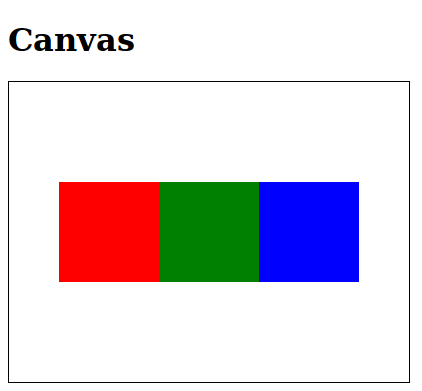
\includegraphics[width=0.7\textwidth]{canvas_ex.png}
\caption{Tre rettangoli disegnati nel canvas}
\label{label:canvasex}
\end{figure}

\section{WebGL: il 3D (realmente) nel Web}
Le prime sperimentazioni di un ``Context'' 3D per l'elemento canvas iniziano nel 2006 all'interno dei laboratori Mozilla ad opera di Vladimir Vukićević\footnote{Corso su WebGL. In \textit{HTML5Today}. Retrieved 12:10, August 14, 2011 from \url{http://www.html5today.it/tutorial/corso-Webgl--introduzione}}. Qualche anno più tardi, nel 2009, visto l'interesse suscitato, fu istituito il \mbox{WebGL} Working Group. Ad oggi è uno standard cross-platform, cross-browser e royalty-free gestito dal consorzio Khronos Group, responsabile anche di altre importanti tecnologie in campo 3D quale, ad esempio, OpenGL. Nel Marzo 2011 è stata rilasciata la versione 1.0 della specifica\footnote{WebGL Specification. In \textit{Khronos Group}. Retrieved 9:20, July 29, 2011 from \url{https://www.khronos.org/registry/Webgl/specs/1.0/}}.

WebGL, acronimo di Web-based Graphics Library, è un'interfaccia di programmazione che consente di creare e gestire contenuti 3D all'interno della pagina Web. Questa libreria espone, per mezzo del tag \texttt{<canvas>}, una DOM API di basso livello, utilizzabile, dunque, attraverso qualsiasi linguaggio ``DOM-compatibile'' (vedi Javascript, Java). Queste caratteristiche consentono di mettere da parte i plugin di terze parti (spesso soluzioni proprietarie) e di accedere ad un 3D "nativo" del Web. Un browser WebGL compatibile si occuperà di fornire l'accelerazione grafica sfruttando l'hardware presente sulla macchina, interfacciandosi direttamente con i driver, con risultati performanti e di alta qualità.

Non a caso infatti WebGL poggia su due tecnologie consolidate e ampiamente diffuse quali OpenGL ES2, API per la grafica 2D e 3D in sistemi embedded (console, telefono, veicoli, etc...), e l'OpenGL Shading Language (GLSL) per la creazione di ``Shader''\footnote{Gli shader sono insiemi di istruzioni, altamente flessibili e riutilizzabili, che definiscono in ogni parte l'aspetto finale che l'oggetto avrà dopo la fase di rendering.}. L'utilizzo di queste tecnolgie fa di WebGL un'interfaccia di basso livello e sebbene da una parte questo porti enormi benefici sul piano dell'efficienza e della qualità, dall'altra introduce un alto livello di complessità, anche per la gestione di contenuti semplicissimi come quelli mostrati in Figura ~\ref{label:spinWebgl}: \textit{``WebGL is a low-level API, so it's not for the faint of heart. OpenGL's shading language, GLSL, is itself an entire programming environment. As a result, even simple things in WebGL take quite a bit of code. You have to load, compile, and link shaders, set up the variables to be passed in to the shaders, and also perform matrix math to animate shapes.''}. Il bagaglio di conoscenze richieste per utilizzare questa tecnologia è enorme come lo sono, di certo, lo sforzo e il tempo richiesti per apprenderle, malgrado questo sia poi il compito di uno sviluppatore.

\begin{figure}[Ht]
\centering
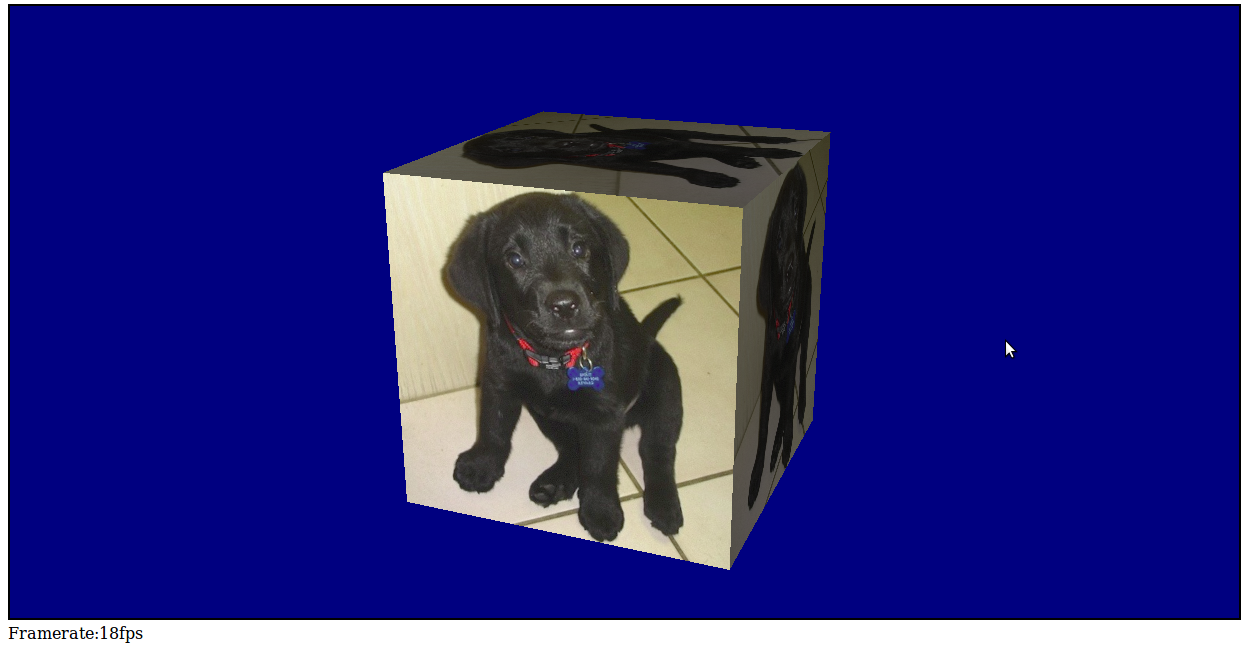
\includegraphics[width=0.7\textwidth]{spinning_webgl.png}
\caption{Cubo con texture in un canvas visualizzato con WebGL}
\label{label:spinWebgl}
\end{figure}

In conclusione WebGL non è uno strumento ``ready-to-use'' e questo potrebbe non giocare a suo favore. Tuttavia, stanno già nascendo librerie di più alto livello che fungono da ``wrapper'' e agevolano la vita al programmatore\footnote{GLGE Official Website. In \textit{GLGE}. Retrieved 7:22, August 18, 2011 from http://www.glge.org/}, mascherando la complessa natura di WebGL e consentendogli dunque di concentrarsi pienamente sulla creazione di contenuti per Web. Tra queste vi è sicuramente X3DOM, un framework che tenta di unire X3D, consolidata tecnologia ``user-friendly'', con l'emergente e complesso WebGL.


\section{X3DOM}
Quanto visto finora con WebgGL consente di introdurre e gestire elementi di grafica 3D nel contesto Web utilizzando un paradigma di programmazione imperativo. Ciò che manca è un modo semplice per integrare in maniera dichiarativa contenuti 3D all'interno del DOM di una pagina HTML. Il percorso iniziato dall'X3D Working Group proponeva X3D per una piena integrazione con HTML5. La scelta di questa tecnologia come base per un 3D dichiarativo appare ovvia, in quanto è uno standard basato su XML, consolidato e assai diffuso tra gli sviluppatori. Inoltre è proprio la specifica HTML5 che nella sua promessa di un ``declarative-3d'' fa riferimento ad X3D, senza specificare però un modello di integrazione. L'obiettivo finale è quello di incorporare una scena X3D all'interno del DOM, come già avvenuto per altri linguaggi XML-based come SVG o MathML, consentendone la manipolazione semplicemente interagendo con i nodi stessi e grazie anche al supporto degli eventi HTML. A questo punto il codice per rappresentare un semplice cubo all'interno di una pagina HTML5 con X3D risulta assi snello e leggibile, come mostra il Listing ~\ref{lst:x3dex}.

\begin{mylisting}{html}{A simple cube with X3D+HTML5}{lst:x3dex}
<!DOCTYPE html>
<html>
<head>
<title>X3D example</title>
<link rel="stylesheet" type="text/css" href="http://www.x3dom.org/x3dom/release/x3dom.css"></link>
<script type="text/javascript" src="http://www.x3dom.org/x3dom/release/x3dom.js"></script>
</head>
<body>
    <h1>X3D - A cube</h1>
    <x3d id='x3d_element' width='880px' height='400px'>
        <scene>
            <shape>
                <appearance>
                    <material diffuseColor='blue'></material>
                </appearance>
                <box></box>
            </shape>
        </scene>
    </x3d>
</body>
</html>
\end{mylisting}

\begin{figure}[Ht]
\centering
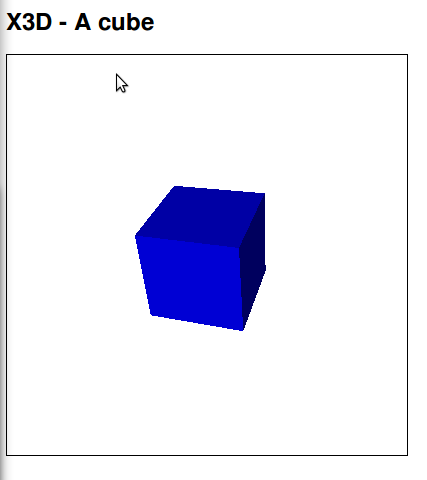
\includegraphics[width=0.7\textwidth]{x3dom_ex.png}
\caption{Un cubo blu realizzato con X3DOM}
\label{label:x3domex}
\end{figure}

Per ottenere il risultato presentato in Figura ~\ref{label:x3domex} dal Listing ~\ref{lst:x3dex} è \mbox{necessario} visualizzare il contenuto X3D della pagina Web. 
Fraunhofer Society, un importante ente di ricerca internazionale, ha lavorato a lungo sia sull'integrazione X3D-HTML5 che sul motore di rendering e il risultato è la suite opensource X3DOM. Questa definisce un modello di integrazione X3D-HTML5 che si può dividere principalmente in due parti: una di interazione con il browser Web e una di comunicazione con l'ambiente X3D in esecuzione. L'architettura di X3DOM consente di supportare diversi frontend, ovvero i browser, e backend, vale a dire le risorse con cui la scena viene rappresentata. Su questo fronte vi sono diverse possibilità, attualmente supportate dalla suite X3DOM: 
\begin{itemize}
	\item Rendering con plugin classico tramite plugin X3D-SAI esterno di terze parti.
	\item Rendering tramite un motore Flash 11, compreso nella suite.
    \item Rendering nativo grazie a WebGL
\end{itemize}
Chiaramente gli sforzi sono concentrati su quest'ultima possibilità, lasciando le prime due opzioni per garantire compatibilità con quei browser che non supportano WebGL o con sistemi obsoleti o privi di accelerazione hardware.

Per poter utilizzare X3DOM basta includere nella nostra pagina Web la componenete javascript \texttt{x3dom.js} e il foglio di stile \texttt{x3dom.css}, come si può notare alle righe 5 e 6 del Listing ~\ref{lst:x3dex}. Sarà questo motore ad occuparsi del recupero della scena X3D dal DOM della pagina, lato frontend, e di sincronizzarla con la rappresentazione della stessa scena lato backend, comunicando, qualora necessario, i cambiamenti in un verso o nell'altro. A seconda del motore di rendering utilizzato, l'engine si preoccuperà di tradurre la scena X3D utilizzando l'interfaccia corretta. Nell'esempio in Figura ~\ref{label:x3domex} viene utilizzata la Canvas 3D API messa a disposizione da WebGL.

Nel capitolo seguente si affronter\`{a} nel dettaglio il software Medea realizzato combinando le tecnologie viste fin qui, allo scopo di metterle alla prova e valutarne la maturità e l'efficienza.
